\documentclass{beamer}
%
% Choose how your presentation looks.
%
% For more themes, color themes and font themes, see:
% http://deic.uab.es/~iblanes/beamer_gallery/index_by_theme.html
%
\mode<presentation>
{
  \usetheme{Boadilla}      % or try Darmstadt, Madrid, Warsaw, ...
  \usecolortheme{beaver} % or try albatross, beaver, crane, ...
  \usefonttheme{default}  % or try serif, structurebold, ...
  \setbeamertemplate{navigation symbols}{}
  \setbeamertemplate{caption}[numbered]
  
} 

\usepackage{xcolor,colortbl}
\usepackage[english]{babel}
\usepackage[utf8x]{inputenc}
\usepackage{courier}
\usepackage{dsfont}
\usepackage{soul}% strikeout
\usepackage{verbatim} 
\usepackage{enumerate}
\usepackage{tikz}
\usepackage{multirow}
\usepackage{bbm}
\usepackage{amsmath}
\usepackage{venndiagram}
\usepackage{epigraph} 
%\usepackage{xcolor}

%\usepackage{enumitem}

\usepackage{hyperref}
\hypersetup{
    colorlinks=true,
    linkcolor=blue,
    filecolor=magenta,      
    urlcolor=cyan,
}

% R stuff!
\usepackage{listings}
\definecolor{codegreen}{rgb}{0,0.6,0}
\definecolor{codegray}{rgb}{0.5,0.5,0.5}
\definecolor{codepurple}{rgb}{0.58,0,0.82}
\definecolor{backcolour}{rgb}{0.95,0.95,0.92}

\lstdefinestyle{mystyle}{
    backgroundcolor=\color{backcolour},    
    commentstyle=\color{codegreen},
    keywordstyle=\color{black},
    numberstyle=\tiny\color{codegray},
    stringstyle=\color{codepurple},
    basicstyle=\ttfamily\footnotesize,
    breakatwhitespace=false,         
    breaklines=true,                 
    captionpos=b,                    
    keepspaces=true,                 
    numbers=left,                    
    numbersep=5pt,                  
    showspaces=false,                
    showstringspaces=false,
    showtabs=false,                  
    tabsize=2
}

\lstset{style=mystyle}



%% Size options for nested itemized lists
\usepackage{relsize}
\setbeamerfont{itemize/enumerate body}{parent=normal text}
\setbeamerfont{itemize/enumerate subbody}{parent=normal text,size=\relsize{-1}}
%\setbeamerfont{itemize/enumerate subsubbody}{parent=normal text,size=\relsize{-1}}




\setbeamertemplate{enumerate items}[default]
\setbeamertemplate{itemize item}[triangle]

%\setitemize{label=\usebeamerfont*{itemize item}%
%  \usebeamercolor[fg]{itemize item}
%  \usebeamertemplate{itemize item}}


\usetikzlibrary{shapes,decorations,arrows,calc,arrows.meta,fit,positioning}
\tikzset{
    -Latex,auto,node distance =1 cm and 1 cm,semithick,
    state/.style ={ellipse, draw, minimum width = 0.7 cm},
    point/.style = {circle, draw, inner sep=0.04cm,fill,node contents={}},
    bidirected/.style={Latex-Latex,dashed},
    el/.style = {inner sep=2pt, align=left, sloped}
}

\newcommand{\Mypm}{\mathbin{\tikz [x=1.4ex,y=1.4ex,line width=.1ex] \draw (0.0,0) -- (1.0,0) (0.5,0.08) -- (0.5,0.92) (0.0,0.5) -- (1.0,0.5);}}%



%% For block quote
\usepackage{etoolbox}
\AtBeginEnvironment{quote}{\par\singlespacing\small}



\title[Introduction to Statistics]{Hypothesis Testing pt. 6}
\subtitle{More on Difference Tests for Means}
\author{Grinnell College}
\date{}

\graphicspath{{img/}}

\begin{document}

\begin{frame}
  \titlepage
\end{frame}

%%%%%%%%%%%%%%%%%%%%%%%%%%%%%%%%%%%%%%%%%%%%%%%%%%%%%%%%%%%%%%%
\begin{frame}{Review -- Testing}
Hypothesis Testing Procedure
\begin{enumerate}
\item Construct null and alternate hypotheses, $H_0$ and $H_A$
\item Collect data and compute our sample statistic (i.e., $\overline{x}$)
\item Evaluate that statistic in the context of a null distribution, i.e., 
\begin{align*}
T = \frac{\overline{x} - \mu_0}{\hat{\sigma}/\sqrt{n}} \sim t_{df=n-1}
\end{align*}
\item Reject or fail to reject hypothesis
\begin{itemize}
\item Type I errors (false positive)
\item Type II errors (false negative)
\end{itemize}
\end{enumerate}
\end{frame}

%%%%%%%%%%%%%%%%%%%%%%%%%%%%%%%%%%%%%%%%%%%%%%%%%%%%%%%%%%%%%%%
\begin{frame}{Review -- Group Differences}
Often in statistical inference, we are interested in investigating the \textit{difference} between two or more groups \vspace{4mm}

For example, we may have two groups, $A$ and $B$, with a mean value for each group, $\mu_A$ and $\mu_B$ \\ \vspace{4mm}

Expressed in our null hypothesis, this equates to
\begin{align*}
H_0: \mu_A = \mu_B \quad \text{or} \quad H_0: \mu_A - \mu_B = 0
\end{align*}
\end{frame}


%%%%%%%%%%%%%%%%%%%%%%%%%%%%%%%%%%%%%%%%%%%%%%%%%%%%%%%%%%%%%%%
\begin{frame}{Two-sampled t-test}

There are a number of various assumptions we can make about the data for testing diff. in means, all resulting in slightly different tests (degrees of freedom and standard error): \vspace{5mm}

\begin{enumerate}
\item Independent, groups same size and have same variance
\item Independent, groups have unequal sizes and similar variance
\item Independent, groups have different sizes and different variances
\item Paired testing
\end{enumerate}

\vspace{5mm}

Of (1), (2), and (3)... (3) is the most versatile. \vspace{2mm}

In general, we will concern ourselves with (3) and (4)

\end{frame}

%%%%%%%%%%%%%%%%%%%%%%%%%%%%%%%%%%%%%%%%%%%%%%%%%%%%%%%%%%%%%%%
\begin{frame}{Two-sampled t-test}

There are a number of various assumptions we can make about the data for testing diff. in means, all resulting in slightly different tests (degrees of freedom and standard error): \vspace{5mm}

\begin{enumerate}
\item \st{Independent, groups same size and have same variance}
\item \st{Independent, groups have unequal sizes and similar variance}
\item Independent, groups have different sizes and different variances
\item Paired testing
\end{enumerate}

\vspace{5mm}

Of (1), (2), and (3)... (3) is the most versatile. \vspace{2mm}

In general, we will concern ourselves with (3) and (4)

\end{frame}

\begin{frame}{Review -- Hypothesis Test for Difference of Means}
H$_0$: $\mu_1 - \mu_2 = \mu_0$ = 0 \vspace{3mm}

\textbf{Conditions:}
\begin{itemize}
    \item Random Sample
    \item Normal population \textbf{OR} $n_1 \geq$ 30 and $n_2 \geq 30$
\end{itemize} \vspace{3mm}


\textbf{When $\sigma$ is not known:}
\begin{equation*}
    T := \frac{\bar{x}_1-\bar{x}_2}{\sqrt{\frac{s_1^2}{n_1}+\frac{s_2^2}{n_2}}} \sim \textbf{t(df = min($n_1$, $n_2$) - 1)}
\end{equation*} \vspace{-4mm}
\begin{itemize}
    \item use pt() function with value of T and df
\end{itemize}
\end{frame}

%%%%%%%%%%%%%%%%%%%%%%%%%%%%%%%%%%%%%%%%%%%%%%%%%%%%%%%%%%%%%%%
\begin{frame}{Degrees of Freedom}
With our test-statistic from above:
\begin{equation*}
    T := \frac{\bar{x}_1-\bar{x}_2}{\sqrt{\frac{s_1^2}{n_1}+\frac{s_2^2}{n_2}}} \sim t_{df},
\end{equation*}
there is actually controversy over how to calculate the df for this \vspace{8mm}

\textbf{Option 1:} df = $min(n_1, n_2)-1$ is the most \textit{conservative} option
\begin{itemize}
    \item gives us largest p-value, and thus weakest evidence of the 3 options
    \item simple: use this if you don't have access to computer for Option 3
\end{itemize} \vspace{6mm}

\textbf{Option 2:} df = $n_1 + n_2 - 2$ is the least conservative
\begin{itemize}
    \item gives us smallest p-value, and thus strongest evidence of the 3 options
    \item relies on assumption of $\sigma_1 = \sigma_2$ (how do we know this?)
\end{itemize}
\end{frame}

%%%%%%%%%%%%%%%%%%%%%%%%%%%%%%%%%%%%%%%%%%%%%%%%%%%%%%%%%%%%%%%
\begin{frame}{Degrees of Freedom}
With our test-statistic from above:
\begin{equation*}
    T := \frac{\bar{x}_1-\bar{x}_2}{\sqrt{\frac{s_1^2}{n_1}+\frac{s_2^2}{n_2}}} \sim t_{df},
\end{equation*}
there is actually controversy over how to calculate the df for this \vspace{6mm}

\textbf{Option 3:} Satterthwaite Approximation
\begin{center}
    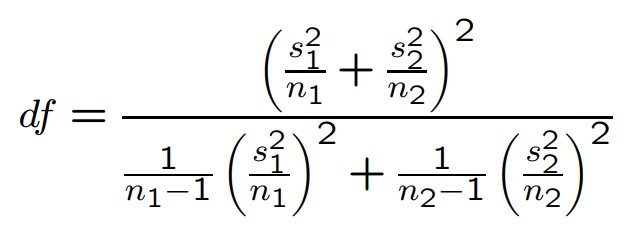
\includegraphics[scale=.6]{img/satterthwaite_df_approx.jpg}
\end{center}

\begin{itemize}
    \item closest to the truth, but fractional value and hard to interpret!
    \item df will be inbetween values for the other options
    \item when we use R to do a t-test later on, look for fractional values of df
\end{itemize}
\end{frame}

%%%%%%%%%%%%%%%%%%%%%%%%%%%%%%%%%%%%%%%%%%%%%%%%%%%%%%%%%%%%%%%
\begin{frame}{Example -- College data}
Consider our college data, where we might investigate the differences in median debt upon graduate for public and private schools



\begin{columns}

  \begin{column}{0.45\textwidth}
\begin{itemize}
\item Private Schools
\begin{itemize}
\item $\overline{x}_1 = 18028$
\item $\hat{\sigma}_1 = 3995$
\item $n_1 = 647$
\end{itemize}
\item Public Schools
\begin{itemize}
\item $\overline{x}_2 = 15627$
\item $\hat{\sigma}_2 = 3111$
\item $n_2 = 559$
\end{itemize}
\end{itemize}
  \end{column}
  \begin{column}{0.5\textwidth}
\begin{center}
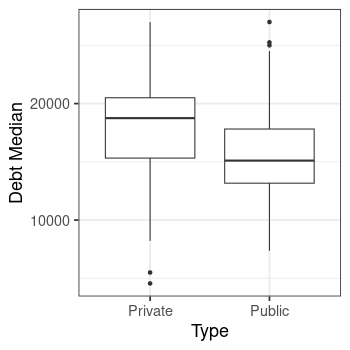
\includegraphics[scale=0.5]{debt_plot.png}
\end{center}
  \end{column}
\end{columns}
\end{frame}

\begin{frame}[fragile]{Example -- College Data}
\small

Again, we will use R to compute this, utilizing a special ``formula" syntax when using data.frames (will cover in lab)


\begin{lstlisting}[language=R]
> t.test(Debt_median ~ Private, college)

	Welch Two Sample t-test

data:  Debt_median by Private
t = 11.2, df = 1075, p-value <0.0000000000000002
alternative hypothesis: true difference in means between group Private and group Public is not equal to 0
95 percent confidence interval:
 1981.0 2820.6
sample estimates:
mean in group Private 
                18028 
 mean in group Public 
                15627 
\end{lstlisting}
\begin{itemize}
    \item min(n1,n2)-1 = 559 - 1 = 558
    \item n1 + n2 - 2 = 647 + 559 = 1206
\end{itemize}

\end{frame}


%%%%%%%%%%%%%%%%%%%%%%%%%%%%%%%%%%%%%%%%%%%%%%%%%%%%%%%%%%%%%%%
\begin{frame}{Paired t-test}
The \textbf{paired t-test} or \textbf{paired difference test} is a test for assessing differences in group means where the groups consist of the same subjects with multiple observations \vspace{4mm}

While you may want to treat this as a two-sample t-test, in practice it more closely resembles that of a one-sample test:

\begin{align*}
T_{\text{paired}} = \frac{\overline{x}_d - \mu_0}{\hat{\sigma}_d / \sqrt{n}}
\end{align*}

where $n$ represents the number of \textit{unique} subjects and $\overline{x}_d$ and $\hat{\sigma}_d$ represent the mean and standard deviation of the \textit{differences} between observations for each subject
\end{frame}


%%%%%%%%%%%%%%%%%%%%%%%%%%%%%%%%%%%%%%%%%%%%%%%%%%%%%%%%%%%%%%%
\begin{frame}{Paired t-test}
Just as with the unpaired case, our null hypothesis is typically that
\begin{align*}
H_0: \mu_d := \mu_1 - \mu_2 = \mu_0 = 0
\end{align*}

Paired testing between groups allows us to control for within-subject variation, effectively reducing variation and making it easier to detect a true difference (power) \vspace{4mm}

This comes at a cost, however -- for $n$ subjects we are required to make $2n$ unique observations
\end{frame}


%%%%%%%%%%%%%%%%%%%%%%%%%%%%%%%%%%%%%%%%%%%%%%%%%%%%%%%%%%%%%%%
\begin{frame}{Example -- French Institute}
Consider the results of a summer institute program sponsored by the National Endowment for the Humanities to improve language abilities in foreign language high school teachers \vspace{4mm}

Twenty teachers were given a listening test of spoken French before and after the program, with a maximum score of 36. We are interested in determining the efficacy of the summer institute \vspace{10mm}

\begin{enumerate}
\item What is the null hypothesis for this study?
\begin{itemize}
\item What would be a Type I error?
\item A Type II error?
\end{itemize}
\item How many total subjects do we have?
\item How many recorded observations do we have?
\end{enumerate}
\end{frame}


%%%%%%%%%%%%%%%%%%%%%%%%%%%%%%%%%%%%%%%%%%%%%%%%%%%%%%%%%%%%%%%
\begin{frame}{Example -- French Institute}
\small
The results of the tests are as follows:
% latex table generated in R 4.3.3 by xtable 1.8-4 package
% Sun Apr 14 11:30:39 2024
\begin{table}[ht]
\centering
\begin{tabular}{rrrr||rrrr}
  \hline
ID & Pretest & Posttest & Difference & ID & Pretest & Posttest & Difference \\ 
  \hline
1 & 32 & 34 & 2 & 11 & 30 & 36 & 6 \\ 
  2 & 31 & 31 & 0 & 12 & 20 & 26 & 6 \\ 
  3 & 29 & 35 & 6 & 13 & 24 & 27 & 3 \\ 
  4 & 10 & 16 & 6 & 14 & 24 & 24 & 0 \\ 
  5 & 30 & 33 & 3 & 15 & 31 & 32 & 1 \\ 
  6 & 33 & 36 & 3 & 16 & 30 & 31 & 1 \\ 
  7 & 22 & 24 & 2 & 17 & 15 & 15 & 0 \\ 
  8 & 25 & 28 & 3 & 18 & 32 & 34 & 2 \\ 
  9 & 32 & 26 & -6 & 19 & 23 & 26 & 3 \\ 
  10 & 20 & 26 & 6 & 20 & 23 & 26 & 3 \\ 
   \hline
\end{tabular}
\end{table}
\end{frame}


%%%%%%%%%%%%%%%%%%%%%%%%%%%%%%%%%%%%%%%%%%%%%%%%%%%%%%%%%%%%%%%
\begin{frame}{Example -- French Institute}
\begin{center}
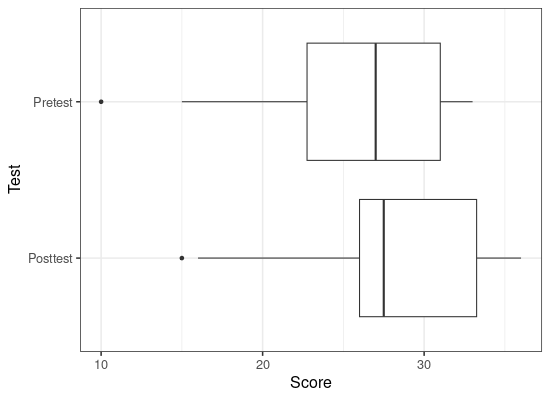
\includegraphics[scale=0.5]{french_prepost.png}
\end{center}
\begin{itemize}
    \item if I do a two-sample t-test for a diff. in means, will I find a difference?
\end{itemize}
\end{frame}

\begin{frame}{Example -- French Institute}
\begin{center}
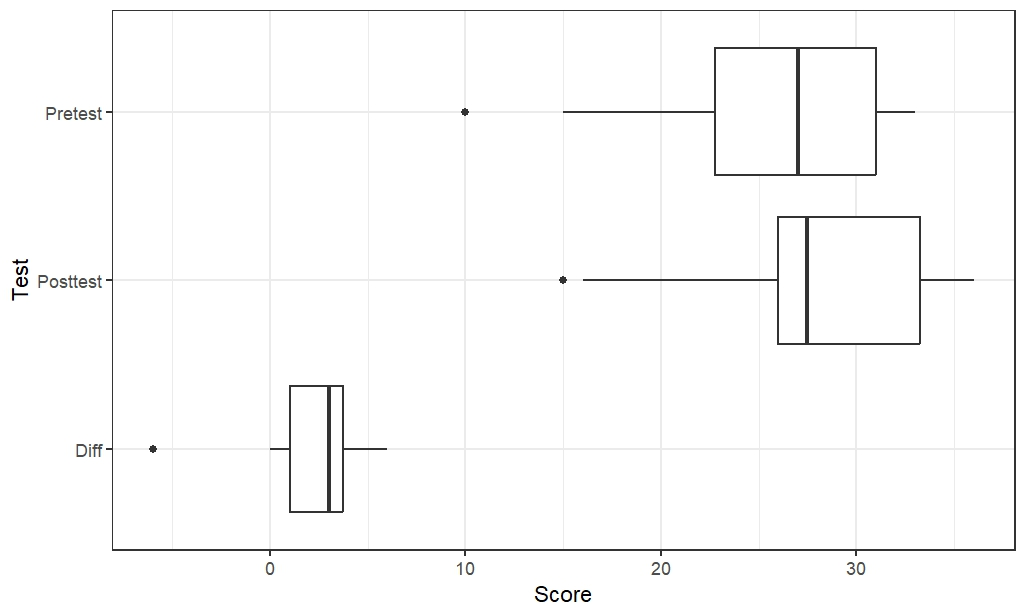
\includegraphics[scale=0.6]{img/diff_plot.jpeg}
\end{center}
\begin{itemize}
    \item If we do a paired t-test to see if differences are zero, what will we find?
\end{itemize}
\end{frame}

%%%%%%%%%%%%%%%%%%%%%%%%%%%%%%%%%%%%%%%%%%%%%%%%%%%%%%%%%%%%%%%
\begin{frame}[fragile]{Example -- French Institute}

Results of the \textit{paired t-test}

\begin{lstlisting}[language=R,basicstyle=\ttfamily\large]
> t.test(post, pre, paired = TRUE)

	Paired t-test

data:  post and pre
t = 3.86, df = 19, p-value = 0.001
alternative hypothesis: true mean difference is not equal to 0
95 percent confidence interval:
 1.1461 3.8539
sample estimates:
mean difference 
            2.5 
\end{lstlisting}
\end{frame}


%%%%%%%%%%%%%%%%%%%%%%%%%%%%%%%%%%%%%%%%%%%%%%%%%%%%%%%%%%%%%%%
\begin{frame}[fragile]{Example -- French Institute}
Results of the unpaired t-test, no power to find difference

\begin{lstlisting}[language=R,basicstyle=\ttfamily\large]
> t.test(post, pre, paired = FALSE)

	Welch Two Sample t-test

data:  post and pre
t = 1.29, df = 37.9, p-value = 0.2
alternative hypothesis: true difference in means is not equal to 0
95 percent confidence interval:
 -1.424  6.424
sample estimates:
mean of x mean of y 
     28.3      25.8 
\end{lstlisting}
\end{frame}

%%%%%%%%%%%%%%%%%%%%%%%%%%%%%%%%%%%%%%%%%%%%%%%%%%%%%%%%%%%%%%%
\begin{frame}{Review}
\begin{itemize}
\item There are different ways of calculating the df for diff. in means test
\item Two-sample t-tests have a paired version
\begin{enumerate}
\item Reduces variability
\item Also reduces degrees of freedom
\item see if you can use paired test by checking if there are multiple observations per subject
\end{enumerate}
\item We can use R to do most of these for us
\begin{itemize}
    \item examples in today's lab
\end{itemize}
\end{itemize}
\end{frame}

%%%%%%%%%%%%%%%%%%%%%%%%%%%%%%%%%%%%%%%%%%%%%%%%%%%%%%%%%%%%%%%
\begin{frame}{Testing Proportions in R}
We can also use R to do the following:
\begin{itemize}
    \item test if a proportion is equal to some value
    \begin{itemize}
        \item $H_0: p = p_0$
    \end{itemize}
    \item test if two (or more!) proportions equal zero
    \begin{itemize}
        \item $H_0: p_1 = p_2$
        \item $H_0: p_1 - p_2 = 0$
        \item $H_0: p_1 = p_2 = ... = p_N$ (N is \# of groups, not sample size)
    \end{itemize}
\end{itemize}
\end{frame}


%%%%%%%%%%%%%%%%%%%%%%%%%%%%%%%%%%%%%%%%%%%%%%%%%%%%%%%%%%%%%%%
\begin{frame}{Difference in Proportions}
% latex table generated in R 4.3.3 by xtable 1.8-4 package
% Sat Apr 13 12:29:32 2024
\begin{table}[ht]
\centering
\begin{tabular}{rrrr}
  \hline
 & Private & Public & Total \\ 
  \hline
Great Lakes & 125 &  64 & 189 \\ 
  Plains &  84 &  42 & 126 \\ 
   \hline
\end{tabular}
\end{table}


\begin{columns}

  \begin{column}{0.45\textwidth}
\begin{itemize}
\item $H_0: p_1 - p_2 = 0$
\item $\hat{p}_1 = 0.661, n_1 = 189$
\item $\hat{p}_2 = 0.666, n_2 = 126$
\item will a test find a difference?
\end{itemize}
  \end{column}
  \begin{column}{0.45\textwidth}
     \begin{center}
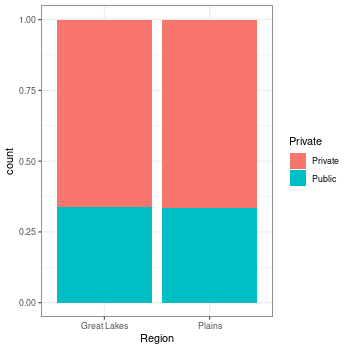
\includegraphics[scale=0.45]{region_private_2.png}
\end{center}
  \end{column}
\end{columns}
\end{frame}

%%%%%%%%%%%%%%%%%%%%%%%%%%%%%%%%%%%%%%%%%%%%%%%%%%%%%%%%%%%%%%%
\begin{frame}{Review -- Hypothesis Test for Difference of Proportions}
H$_0$: $p_1 - p_2$ = 0 \vspace{4mm}

Under $H_0$, $p_1 = p_2$, both are estimating the same thing.
\begin{equation*}
    \text{Let} \hspace{3mm} \widehat{p}_{pool} = \frac{x_1 + x_2}{n_1 + n_2} = \frac{n_1\hat{p}_1 + n_2\hat{p}_2}{n_1 + n_2}
\end{equation*}

If we are simulating what the null hypothesis looks like, then
\begin{equation*}
    Z := \frac{(\hat{p}_1 - \hat{p}_2) - 0}{\sqrt{\frac{\widehat{p}_{pool}(1-\widehat{p}_{pool})}{n_1}+\frac{\widehat{p}_{pool}(1-\widehat{p}_{pool})}{n_2}}} = \frac{(\hat{p}_1 - \hat{p}_2)}{\sqrt{\widehat{p}_{pool}(1-\widehat{p}_{pool})(\frac{1}{n_1}+\frac{1}{n_2})}} \sim \textbf{N(0,1)}
\end{equation*} \vspace{-4mm}
\begin{itemize}
    \item use pnorm() with value of Z
\end{itemize}
\end{frame}


%%%%%%%%%%%%%%%%%%%%%%%%%%%%%%%%%%%%%%%%%%%%%%%%%%%%%%%%%%%%%%%
\begin{frame}[fragile]
\footnotesize

\begin{table}[ht]
\centering
\begin{tabular}{rrrr}
  \hline
 & Private & Public & Total \\ 
  \hline
Great Lakes & 125 &  64 & 189 \\ 
  Plains &  84 &  42 & 126 \\ 
   \hline
\end{tabular}
\end{table}


\begin{lstlisting}[language=R]
> prop.test(x = c(125, 84), n = c(189, 126))

	2-sample test for equality of
	proportions with continuity
	correction

data:  c(125, 84) out of c(189, 126)
X-squared < 3.74E-30
df = 1, p-value = 1
alternative hypothesis: two.sided
95 percent confidence interval:
 -0.11701  0.10643
sample estimates:
 prop 1  prop 2 
0.66138 0.66667 
\end{lstlisting}
\begin{itemize}
    \item The test-statistic R uses here is actually the square of the test-statistic we previously found ($Z^2$)
    \item the distribution is not standard Normal, it is something else that we will talk about on Monday. Regardless, the p-value from `prop.test()` is still the same
\end{itemize}
\end{frame}

%%%%%%%%%%%%%%%%%%%%%%%%%%%%%%%%%%%%%%%%%%%%%%%%%%%%%%%%%%%%%%%




%%%%%%%%%%%%%%%%

%\begin{frame}
%\begin{columns}
%
%  \begin{column}{0.45\textwidth}
%%
%  \end{column}
%  \begin{column}{0.45\textwidth}
%%
%  \end{column}
%
%\end{columns}
%\end{frame}


\end{document}
